\chapter{Two-Dimensional Wannier Reduction: From Separable to Coupled Potentials}
\index{warmup!two-dimensional|textbf}

\label{app:two-dimensional-reduction}

\chapterstatus{human-accepted calculated controlled synthetic
numerical-verification exercise. Exact separable identities, independent plane-wave and real-space
parent refinement, degenerate projectors, reciprocal-loop and topology
diagnostics, scalar and rank-three composite Wannier hoppings, direct
localization diagnostics, shell reduction, tensor masses, a frozen
nonseparable-coupling sequence, and separate Qi--Wu--Zhang, Hofstadter, and
Haldane Chern-band controls have been independently verified. The first
Wannier90 preprocessing attempt failed and is retained; a separately authorized
balanced-embedding attempt converged and was independently reconstructed. Six
additional non-DFT cases retain nonmonotone mesh, cutoff, and embedding
sensitivity, so no converged localization limit is claimed. No material
calculation, scientific validation, or uncertainty quantification is claimed.}

\section{Purpose}

A two-dimensional periodic model is useful if it remains simple enough to
verify while introducing features absent in one dimension. These include a
Brillouin-zone mesh rather than a line, symmetry-related degeneracies,
direction-dependent hopping shells, effective-mass tensors, gauge closure
around reciprocal-space loops, and possible topological obstructions to
Wannier localization.

The proposed parent begins with a separable square-lattice cosine potential.
Its bands and Bloch states factor into products of the one-dimensional problem,
providing a strong reference. A controlled coupling is then introduced to
break separability without changing the lattice. The progression is
\begin{equation}
    \begin{gathered}
        \text{verified separable parent}
        \\
        \downarrow
        \\
        \text{coupled two-dimensional parent}
        \\
        \downarrow
        \\
        \text{Wannier representation}
        \longrightarrow
        \text{finite-range tight binding}.
    \end{gathered}
\end{equation}

The two-dimensional warmup should answer:
\begin{enumerate}
    \item whether real-space and plane-wave Bloch fibers agree over a full
          two-dimensional reciprocal mesh;
    \item whether the separable limit reproduces sums and products of the
          one-dimensional results;
    \item how degeneracies affect band labels and retained-subspace selection;
    \item how direct gauge transport and Wannier90 localization compare in two
          dimensions;
    \item how hopping blocks decay by lattice vector and symmetry shell;
    \item how finite-range TB models converge to isolated- and composite-band
          parent operators; and
    \item how these conclusions change when separability, fourfold symmetry,
          or isotropy is broken in a controlled manner.
\end{enumerate}

\section{Continuum parent family}

Let the square lattice have primitive vectors
\begin{equation}
    \mathbf a_1=a\mathbf e_x,
    \qquad
    \mathbf a_2=a\mathbf e_y,
\end{equation}
and reciprocal scale
\begin{equation}
    G=\frac{2\pi}{a}.
\end{equation}
Define
\begin{equation}
    V(x,y)
    =
    V_x\cos(Gx)
    +
    V_y\cos(Gy)
    +
    V_{xy}\cos(Gx)\cos(Gy).
\end{equation}
The continuum Hamiltonian on $L^2(\mathbb R^2)$ is
\begin{equation}
    \hat H
    =
    -\frac{\hbar^2}{2m}
    \left(
        \frac{\partial^2}{\partial x^2}
        +
        \frac{\partial^2}{\partial y^2}
    \right)
    +
    V(x,y).
\end{equation}
Use the dimensionless controls
\begin{equation}
    \lambda_x=\frac{V_x}{E_G},
    \qquad
    \lambda_y=\frac{V_y}{E_G},
    \qquad
    \lambda_{xy}=\frac{V_{xy}}{E_G},
    \qquad
    E_G=\frac{\hbar^2G^2}{2m}.
\end{equation}
The first Brillouin zone is
\begin{equation}
    -\frac{G}{2}\leq k_x,k_y<\frac{G}{2}.
\end{equation}

For crystal momentum $\mathbf k=(k_x,k_y)$, write
\begin{equation}
    \psi_{n\mathbf k}(\mathbf r)
    =
    e^{i\mathbf k\cdot\mathbf r}
    u_{n\mathbf k}(\mathbf r),
\end{equation}
where $u_{n\mathbf k}$ is periodic on the square cell. The cell-periodic fiber
operator is
\begin{equation}
    \hat H(\mathbf k)
    =
    \frac{1}{2m}
    \left(-i\hbar\nabla+\hbar\mathbf k\right)^2
    +
    V(x,y).
\end{equation}

\section{Separable reference limit}

When
\begin{equation}
    V_{xy}=0,
\end{equation}
the Hamiltonian separates:
\begin{equation}
    \hat H(\mathbf k)
    =
    \hat H_x(k_x)
    \otimes
    \hat I_y
    +
    \hat I_x
    \otimes
    \hat H_y(k_y).
\end{equation}
Consequently, the exact product-form relations are
\begin{align}
    E_{n_xn_y}(k_x,k_y)
    &=
    E_{n_x}^{(x)}(k_x)
    +
    E_{n_y}^{(y)}(k_y),
    \\
    u_{n_xn_y,\mathbf k}(x,y)
    &=
    u_{n_x,k_x}^{(x)}(x)
    u_{n_y,k_y}^{(y)}(y),
\end{align}
up to basis choices within degenerate product subspaces.

These identities make the separable model more than a qualitative warmup. The
one-dimensional parent supplies expected two-dimensional eigenvalues,
projectors, Wannier products, and axis-supported Kronecker-sum hopping
structure. A two-dimensional
construction that fails these checks in the separable limit has not yet
isolated genuinely two-dimensional physics.

For the isotropic case $V_x=V_y$, product states related by
$n_x\leftrightarrow n_y$ may become symmetry degenerate at selected
$\mathbf k$. The stable comparison object is then the degenerate projector,
not an arbitrary ordering of individual eigenvectors.

\section{Plane-wave Bloch representation}

Use reciprocal indices $(p,q)\in\mathbb Z^2$ and basis functions
\begin{equation}
    \langle\mathbf r\mid p,q;\mathbf k\rangle
    =
    \frac{1}{a}
    e^{i[(k_x+pG)x+(k_y+qG)y]}.
\end{equation}
The kinetic matrix is diagonal:
\begin{equation}
    T_{pq,p'q'}(\mathbf k)
    =
    \frac{\hbar^2}{2m}
    \left[
        (k_x+pG)^2+(k_y+qG)^2
    \right]
    \delta_{pp'}\delta_{qq'}.
\end{equation}
The potential couplings are
\begin{align}
    V_{pq,p'q'}
    &=
    \frac{V_x}{2}
    \left(
        \delta_{p,p'+1}+\delta_{p,p'-1}
    \right)
    \delta_{qq'}
    \\
    &\quad+
    \frac{V_y}{2}
    \left(
        \delta_{q,q'+1}+\delta_{q,q'-1}
    \right)
    \delta_{pp'}
    \\
    &\quad+
    \frac{V_{xy}}{4}
    \sum_{s_x=\pm1}
    \sum_{s_y=\pm1}
    \delta_{p,p'+s_x}
    \delta_{q,q'+s_y}.
\end{align}
The separable terms move along one reciprocal axis at a time. The coupling
$V_{xy}$ connects diagonal reciprocal neighbors and therefore provides a
visible algebraic marker of nonseparability.

Retain
\begin{equation}
    -P_x\leq p\leq P_x,
    \qquad
    -P_y\leq q\leq P_y.
\end{equation}
The represented dimension is
\begin{equation}
    N_{\mathrm{PW}}
    =
    (2P_x+1)(2P_y+1).
\end{equation}
Cutoff convergence should be tested independently in the two directions before
an isotropic cutoff is assumed sufficient.

\section{Real-space Bloch representation}

Use an $N_x\times N_y$ grid on one unit cell with spacings
\begin{equation}
    \Delta x=\frac{a}{N_x},
    \qquad
    \Delta y=\frac{a}{N_y}.
\end{equation}
The boundary identifications are
\begin{align}
    \psi(x+a,y)&=e^{ik_xa}\psi(x,y),
    \\
    \psi(x,y+a)&=e^{ik_ya}\psi(x,y).
\end{align}
A centered second-order representation has the Kronecker-sum form
\begin{equation}
    \mathbf T_h(\mathbf k)
    =
    \mathbf T_x(k_x)\otimes\mathbf I_y
    +
    \mathbf I_x\otimes\mathbf T_y(k_y),
\end{equation}
where the boundary entries of $\mathbf T_x$ and $\mathbf T_y$ carry the
corresponding Bloch phases. The represented Hamiltonian is
\begin{equation}
    \mathbf H_h(\mathbf k)
    =
    \mathbf T_h(\mathbf k)
    +
    \operatorname{diag}
    \left(
        V(x_i,y_j)
    \right).
\end{equation}

At $V_{xy}=0$, this matrix should equal the Kronecker sum of the corresponding
one-dimensional represented Hamiltonians, subject to one fixed vectorization
order. Its eigenvalues should be sums of one-dimensional represented
eigenvalues. This is an exact matrix-level check for the declared discretization,
not merely a continuum expectation.

A two-dimensional discrete Bloch--Fourier transform transports the real-space
matrix into reciprocal coordinates. When
\begin{equation}
    N_x=2P_x+1,
    \qquad
    N_y=2P_y+1,
\end{equation}
the transform is the Kronecker product of the one-dimensional transforms:
\begin{equation}
    \mathbf F_{2\mathrm D}(\mathbf k)
    =
    \mathbf F_x(k_x)\otimes\mathbf F_y(k_y).
\end{equation}
The transported matrix
\begin{equation}
    \mathbf A_h^{\mathrm{FD}\rightarrow\mathrm{PW}}(\mathbf k)
    =
    \mathbf F_{2\mathrm D}(\mathbf k)^\dagger
    \mathbf H_h(\mathbf k)
    \mathbf F_{2\mathrm D}(\mathbf k)
\end{equation}
can be compared with the plane-wave Galerkin matrix in a common basis.
Low-reciprocal-sector and retained-band comparisons should accompany any
full-space Frobenius norm because high-frequency grid modes can dominate the
latter.

\section{Symmetry and degeneracy diagnostics}

For a real scalar potential,
\begin{equation}
    E_n(-\mathbf k)=E_n(\mathbf k)
\end{equation}
under consistent band or subspace matching. In the isotropic separable case,
the square-lattice point symmetries imply additional relations among
$\mathbf k$, rotated momenta, and reflected momenta. The usual high-symmetry
points may be denoted
\begin{equation}
    \Gamma=(0,0),
    \qquad
    X=\left(\frac{G}{2},0\right),
    \qquad
    M=\left(\frac{G}{2},\frac{G}{2}\right).
\end{equation}
A plotted $\Gamma$--$X$--$M$--$\Gamma$ path is useful for visualization but is
not sufficient for Wannier localization or two-dimensional operator norms. The
full reciprocal mesh and its neighbor relations remain required.

At degeneracies, individual eigenvectors are not uniquely defined. Comparisons
should use the projector onto the complete degenerate or nearly degenerate
cluster. Principal angles and overlap singular values determine whether two
represented clusters span the same subspace before an internal gauge is
selected.

Breaking $V_x=V_y$ while retaining $V_{xy}=0$ supplies a controlled anisotropic
case. Turning on $V_{xy}$ supplies a controlled nonseparable case. These two
changes should not be introduced simultaneously in the first comparison.

\section{Effective-mass tensor}
\index{effective-mass tensor}


At an isolated band extremum $\mathbf k_0$, define the inverse effective-mass
tensor
\begin{equation}
    \left(m_n^{\ast-1}\right)_{ij}
    =
    \frac{1}{\hbar^2}
    \left.
        \frac{\partial^2E_n(\mathbf k)}
        {\partial k_i\partial k_j}
    \right|_{\mathbf k=\mathbf k_0}.
\end{equation}
For the separable parent, the mixed derivative should vanish in the lattice
axes, and the diagonal terms should agree with the corresponding
one-dimensional curvatures. In the isotropic case, symmetry may force equal
diagonal entries at selected extrema. These are expected structural checks,
not calculated findings.

The reciprocal stencil, fit region, symmetry constraints, and units must be
held fixed when plane-wave, real-space, Wannier, and TB representations are
compared. A band-path curvature alone does not determine the full tensor.

\section{Direct two-dimensional gauge construction}

For an isolated band, neighboring overlaps are
\begin{equation}
    M^{(\mathbf k,\mathbf b)}
    =
    \langle
        u_{\mathbf k}
        \mid
        u_{\mathbf k+\mathbf b}
    \rangle.
\end{equation}
Parallel transport can be performed along one reciprocal direction on each
mesh line, followed by transport between lines. Unlike the one-dimensional
case, closing the gauge along one direction does not automatically close it
along the other. Wilson loops around reciprocal cycles and elementary mesh
plaquettes diagnose the accumulated holonomy.

For a composite $M$-band subspace, replace each scalar overlap by
\begin{equation}
    \mathbf M^{(\mathbf k,\mathbf b)}_{mn}
    =
    \langle
        u_{m\mathbf k}
        \mid
        u_{n,\mathbf k+\mathbf b}
    \rangle.
\end{equation}
Polar or singular-value decompositions supply neighboring unitary transport
maps. Small singular values identify subspace mismatch or inadequate reciprocal
resolution. A sequence of locally optimal rotations need not produce a globally
periodic and localized frame; loop closure remains an independent condition.

The direct construction should retain every chosen spanning path, overlap,
polar factor, loop holonomy, and closure transformation. Its purpose is not to
replace a mature localization procedure, but to make the gauge problem visible
before it is delegated.

Polar decomposition supplies the nearest unitary factor under the standard
matrix-norm formulation, while its use in Wannier gauge transport and the need
for global reciprocal-space consistency are established in the modern Wannier
literature~\cite{higham1986,marzari2012}.

\section{Topology and the localization boundary}
\index{topology!Wannier localization}


A globally smooth periodic frame for an isolated or composite two-dimensional
subspace can be obstructed by nontrivial topology. The first Chern number may
be written schematically as
\begin{equation}
    C
    =
    \frac{1}{2\pi}
    \int_{\mathrm{BZ}}
    \operatorname{Tr}\boldsymbol{\Omega}(\mathbf k)\,d^2k,
\end{equation}
where $\boldsymbol{\Omega}$ is the Berry-curvature matrix of the retained subspace.
A nonzero $C$ obstructs a complete set of exponentially localized Wannier
functions spanning that subspace.

For periodic insulating subspaces, the relationship between vanishing Chern
invariants, analytic quasi-Bloch functions, and exponentially localized Wannier
functions is treated by Brouder et al.~\cite{brouder2007}. The retained scalar
exercise checks only the expected trivial case and does not test the obstructed
case.

The proposed real scalar cosine family has spinless time-reversal symmetry and
is intended as a topologically trivial starting point. That expectation should
be checked through gauge closure or a discretized curvature diagnostic rather
than inferred from a visually smooth band plot. Degeneracies can also make an
individual-band Chern number undefined until a composite retained subspace is
chosen.

This appendix does not propose introducing magnetic phases or a Chern-band model in
the initial experiment. Topological obstruction is included as a stopping
condition and interpretive lesson, not as a target phenomenon.

\section{Wannier90 localization in two dimensions}

Wannier90 can consume the two-dimensional model Bloch states through the same
general interfaces used in Note~5. The required data include:
\begin{enumerate}
    \item eigenvalues on a uniform $N_{k_x}\times N_{k_y}$ mesh;
    \item neighboring-state overlap matrices in both reciprocal directions;
    \item optional trial-orbital projections;
    \item the square or rectangular lattice convention;
    \item retained band and Wannier counts; and
    \item consistent reciprocal-boundary sewing.
\end{enumerate}
These data correspond to the standard \texttt{.eig}, \texttt{.mmn}, optional
\texttt{.amn}, and \texttt{.win} Wannier90 surfaces~\cite{pizzi2020}.

A formally three-dimensional lattice representation may use one reciprocal
point in an inactive transverse direction. The auxiliary lattice vector and
transverse orbital factor are then representation choices. Active-plane centers
and spreads must be separated from artificial transverse contributions. The
model remains two dimensional even though the localization interface uses a
three-vector lattice convention.

For an isolated band, trial projections may be unnecessary when the direct
parallel-transport gauge is already smooth and periodic. For a composite or
entangled group, projections and possibly disentanglement windows become
material choices~\cite{souza2001}. Projection, disentanglement, gauge rotation,
localization, and hopping truncation must remain separately identified.

The direct and Wannier90 routes should consume the same parent eigenvectors,
mesh, subspace, and overlap matrices. After translations, orbital labels, and
unitary freedom are aligned, compare:
\begin{enumerate}
    \item retained projectors;
    \item Wilson-loop or center phases;
    \item active-plane Wannier centers and spreads;
    \item real-space profiles and symmetry relations;
    \item interpolated bands on withheld $\mathbf k$ points;
    \item aligned real-space Hamiltonian blocks; and
    \item sensitivity to trial projections and mesh refinement.
\end{enumerate}

\section{Two-dimensional Wannier Hamiltonian}

Let $N_k=N_{k_x}N_{k_y}$ and choose one fundamental set
$\mathcal R_{N_k}$ containing exactly $N_k$ lattice-vector representatives
\begin{equation}
    \mathbf R=r_x\mathbf a_1+r_y\mathbf a_2
\end{equation}
modulo the two Born--von Karman superlattice vectors. For a retained $M$-band
frame, define the represented real-space blocks
\begin{equation}
    \mathbf H_{\mathrm W}(\mathbf R)
    =
    \frac{1}{N_k}
    \sum_{\mathbf k}
    e^{-i\mathbf k\cdot\mathbf R}
    \mathbf H_{\mathrm W}(\mathbf k),
    \qquad
    \mathbf R\in\mathcal R_{N_k}.
\end{equation}
The inverse discrete transform is
\begin{equation}
    \mathbf H_{\mathrm W}(\mathbf k)
    =
    \sum_{\mathbf R\in\mathcal R_{N_k}}
    e^{i\mathbf k\cdot\mathbf R}
    \mathbf H_{\mathrm W}(\mathbf R).
\end{equation}
The infinite-lattice interpretation is recovered only through a controlled
reciprocal-mesh limit; periodic copies of one finite-transform coefficient must
not be counted as independent hoppings.

In the separable isolated-product case, the two-dimensional Wannier functions
should factor into one-dimensional Wannier functions up to gauge choices within
degenerate product spaces. The Hamiltonian contains axis-directed contributions
inherited from the one-dimensional factors. Any unexpected diagonal or mixed
hopping should first be checked against gauge mixing, degeneracy, transform
conventions, and aliasing.

The coupled term $V_{xy}$ generally destroys product factorization and can
produce genuine mixed-direction structure in the retained representation. Its
controlled onset provides a direct test of whether the localization and
hopping analysis detects nonseparability.

\section{Two-dimensional tight-binding hierarchy}
\index{tight-binding model!two-dimensional}


Choose a retained set
\begin{equation}
    \mathcal R_c\subseteq\mathcal R_{N_k}
\end{equation}
of distinct Born--von Karman representatives. The finite-range model is
\begin{equation}
    \mathbf H_{\mathrm{TB}}^{(\mathcal R_c)}(\mathbf k)
    =
    \sum_{\mathbf R\in\mathcal R_c}
    e^{i\mathbf k\cdot\mathbf R}
    \mathbf H_{\mathrm W}(\mathbf R).
\end{equation}
In two dimensions, ``range'' is not unique. Possible hierarchies include:
\begin{enumerate}
    \item Euclidean-distance shells;
    \item Manhattan-distance shells;
    \item square-lattice point-group orbits; and
    \item physically declared neighbor shells.
\end{enumerate}
The hierarchy must be frozen before outcomes are inspected. A symmetry shell
should be retained or omitted as a complete orbit when the model class is
claimed to preserve that symmetry.

The omitted-block residual is
\begin{equation}
    \Delta\mathbf H^{(\mathcal R_c)}(\mathbf k)
    =
    \sum_{\mathbf R\in\mathcal R_{N_k}\setminus\mathcal R_c}
    e^{i\mathbf k\cdot\mathbf R}
    \mathbf H_{\mathrm W}(\mathbf R).
\end{equation}
For a complete uniform transform, Parseval's identity relates the full-mesh
reciprocal Frobenius residual to the omitted real-space block norm:
\begin{equation}
    \sum_{\mathbf k}
    \left\lVert
        \Delta\mathbf H^{(\mathcal R_c)}(\mathbf k)
    \right\rVert_{\mathrm F}^2
    =
    N_k
    \sum_{\mathbf R\in\mathcal R_{N_k}\setminus\mathcal R_c}
    \left\lVert
        \mathbf H_{\mathrm W}(\mathbf R)
    \right\rVert_{\mathrm F}^2.
\end{equation}
Nonuniform reciprocal weights or incomplete transforms define a different
objective.

\section{Direct and mediated reduction routes}

The mediated route constructs $\mathbf H_{\mathrm W}(\mathbf R)$ and truncates
or fits it within a declared shell hierarchy. The direct route fits the same
finite-dimensional model class to parent band data over selected reciprocal
points.

For one isolated band, a complete uniform mesh, equal weights, and an
unconstrained set of retained lattice Fourier coefficients that are distinct
modulo the Born--von Karman superlattice, direct least squares and mediated
Fourier truncation are expected to agree. In a composite subspace,
the direct spectral objective does not identify a unique matrix-valued operator
because momentum-dependent unitary rotations preserve the eigenvalues. An
aligned operator objective or additional orbital information is required.

The route defect is
\begin{equation}
    D_{\mathrm{path}}^2
    =
    \sum_{\mathbf k\in\mathcal K_{\mathrm{cmp}}}
    w_{\mathbf k}
    \left\lVert
        \mathbf H_{\mathrm{TB,dir}}(\mathbf k)
        -
        \mathbf C(\mathbf k)^\dagger
        \mathbf H_{\mathrm{TB,med}}(\mathbf k)
        \mathbf C(\mathbf k)
    \right\rVert_{\mathrm F}^2,
\end{equation}
where $\mathbf C(\mathbf k)$ is an admissible periodic alignment when the
final orbital conventions differ. A constant cell-local matrix is sufficient
only when the two gauges differ by a momentum-independent orbital rotation. A
general momentum-dependent alignment can mix real-space cells and change the
apparent hopping range, so its smoothness, periodicity, and real-space action
must be retained with the route comparison. The comparison should vary
reciprocal weighting, withheld regions, shell constraints, gauge choices, and
composite rank one at a time.

\section{Staged method and execution status}

The retained calculation executes the separable and parent-convergence stages,
lowest-band reciprocal-loop and Chern diagnostics, symmetry-shell truncation,
matched direct-versus-mediated reduction, and the frozen nonseparable-coupling
continuation. Degeneracy is tested through a rank-two projector control. A
human-requested extension adds a direct rank-three projected-gauge and
localization comparison. Three separate topological models then test nonzero
Chern and Wilson-winding diagnostics without identifying any model with the
scalar parent. The first authorized Wannier90 attempt failed during
preprocessing; the separately authorized balanced-embedding correction then
converged and supplies the independent external localization comparison.

\subsection{Stage A: reproduce the separable product structure}

Set $V_{xy}=0$. For selected $(V_x,V_y)$, compare two-dimensional plane-wave
and real-space eigenvalues and projectors with sums and products of converged
one-dimensional results. Verify Kronecker-sum identities at the represented
matrix level and treat symmetry degeneracies as complete subspaces.

\subsection{Stage B: converge the two parent representations}

Refine $(P_x,P_y)$ and $(\Delta x,\Delta y)$ independently over a full frozen
reciprocal mesh. Compare low-sector transported operators, band energies,
projectors, symmetry residuals, gaps, bandwidths, and effective-mass tensors.
Freeze neither parent representation until the declared quantities are stable
under both routes.

\subsection{Stage C: construct direct two-dimensional gauges}

For an isolated band, perform parallel transport along reciprocal lines, record
loop holonomies, and impose periodic closure in both directions. For a
composite subspace, use overlap polar factors and Wilson loops. Retain overlap
singular values and stop if the selected subspace is not compatible across the
mesh.

\subsection{Stage D: compare with Wannier90}

Provide Wannier90 with the same eigenvalues, overlap matrices, reciprocal mesh,
and optional projections. Compare direct and Wannier90 centers, active-plane
spreads, projectors, profiles, interpolated bands, and aligned hopping blocks.
Repeat under mesh refinement and controlled projection changes.

\subsection{Stage E: verify topology and symmetry}

Evaluate reciprocal-loop closure and a discretized Berry-curvature or Chern
diagnostic for the retained subspace. Verify the expected trivial starting
case before interpreting localization. Check square-lattice symmetry in the
isotropic model and its controlled reduction in the anisotropic model.

\subsection{Stage F: truncate by two-dimensional hopping shell}

Freeze a symmetry-respecting shell hierarchy. At each level report omitted
block norms, reciprocal operator residuals, training and withheld band errors,
gaps, bandwidths, and effective-mass-tensor errors. Compare Euclidean and
physically declared shell orderings only as separately named model classes.

\subsection{Stage G: compare direct and mediated reductions}

Begin with an isolated band and complete uniform reciprocal data, where route
agreement is expected. Then introduce composite bands, withheld reciprocal
regions, nonuniform weights, symmetry-constrained shells, and independent gauge
choices one at a time. Align final operators before forming the route defect.

\subsection{Stage H: turn on nonseparable coupling}

Increase $\lambda_{xy}$ from zero through a frozen sequence while holding the
remaining controls fixed. At each value repeat parent convergence, subspace,
localization, hopping-decay, and route comparisons. Determine which observed
changes are physical consequences of coupling and which arise from lost
numerical convergence or a changed retained manifold.

\section{Error accounting}

The proposed experiment should retain separately:
\begin{enumerate}
    \item one-dimensional reference error inherited by the separable check;
    \item two-dimensional plane-wave cutoff error;
    \item real-space grid and stencil error in each direction;
    \item reciprocal-mesh and interpolation error;
    \item symmetry and degeneracy-cluster matching error;
    \item retained-subspace and overlap-conditioning error;
    \item loop-closure, gauge, and topology diagnostics;
    \item direct-versus-Wannier90 localization discrepancy;
    \item hopping-shell truncation error;
    \item direct-fit optimization and identifiability error;
    \item effective-mass-tensor extraction error; and
    \item nonseparable-coupling continuation error.
\end{enumerate}
No scalar total error is defined. The experiment is an illustrative numerical
verification problem, not scientific validation of a two-dimensional material
or of silicon.

\section{Calculated result}

The retained input fixes $\lambda_x=\lambda_y=0.5$ and varies
$\lambda_{xy}=0,0.05,0.15,0.30$. The represented separable Kronecker-sum defect
is exactly zero, the complete product-spectrum defect is
$3.55\times10^{-14}E_G$, and the rank-two product-projector defect is
$8.08\times10^{-14}$. A controlled internal $45^\circ$ rotation reduces
individual-state overlap to $1/\sqrt{2}$ while changing the projector by only
$2.68\times10^{-16}$.

For the coupled parent at $\lambda_{xy}=0.15$, the maximum lowest-four-band
plane-wave cutoff error decreases from $5.25\times10^{-2}E_G$ at $P=1$ to
$6.27\times10^{-11}E_G$ at $P=4$ relative to $P=5$. The independent
finite-difference sequence decreases monotonically to a
$6.27\times10^{-3}E_G$ spectral error and a $5.34\times10^{-2}E_G$ transported
low-sector operator defect at $25^2$ points. These remain distinct parent
errors rather than being combined.

Across the coupling sequence, the minimum isolation gap decreases from
$0.4971E_G$ to $0.3251E_G$, while sewn neighboring overlaps remain above
$0.978$. The lattice Chern diagnostic is zero, the Wilson phases have no
transverse winding, and a deterministic momentum-dependent phase attack changes
the retained loop diagnostics by at most $1.14\times10^{-15}$. This verifies the
expected trivial scalar family; it does not test a topological obstruction.

Mixed-direction hopping grows from a $3.00\times10^{-15}E_G$ numerical floor at
the separable point to $1.94\times10^{-3}E_G$ at
$\lambda_{xy}=0.30$. Matched direct and mediated shell coefficients agree
within $3.37\times10^{-16}E_G$. The complete finite transform reconstructs the
$15\times15$ mesh to binary64 precision, but the strongest-coupling
$31\times31$ withheld error remains $1.70\times10^{-6}E_G$; reciprocal-mesh
interpolation and hopping truncation are therefore separate limits. The
isotropic principal mass changes from $1.534m$ to $1.313m$. A separate
anisotropic control gives $1.184m$ and $2.112m$ while retaining time reversal
and reflection and deliberately breaking fourfold rotation by
$7.46\times10^{-2}E_G$.

\begin{figure}[p]
  \centering
  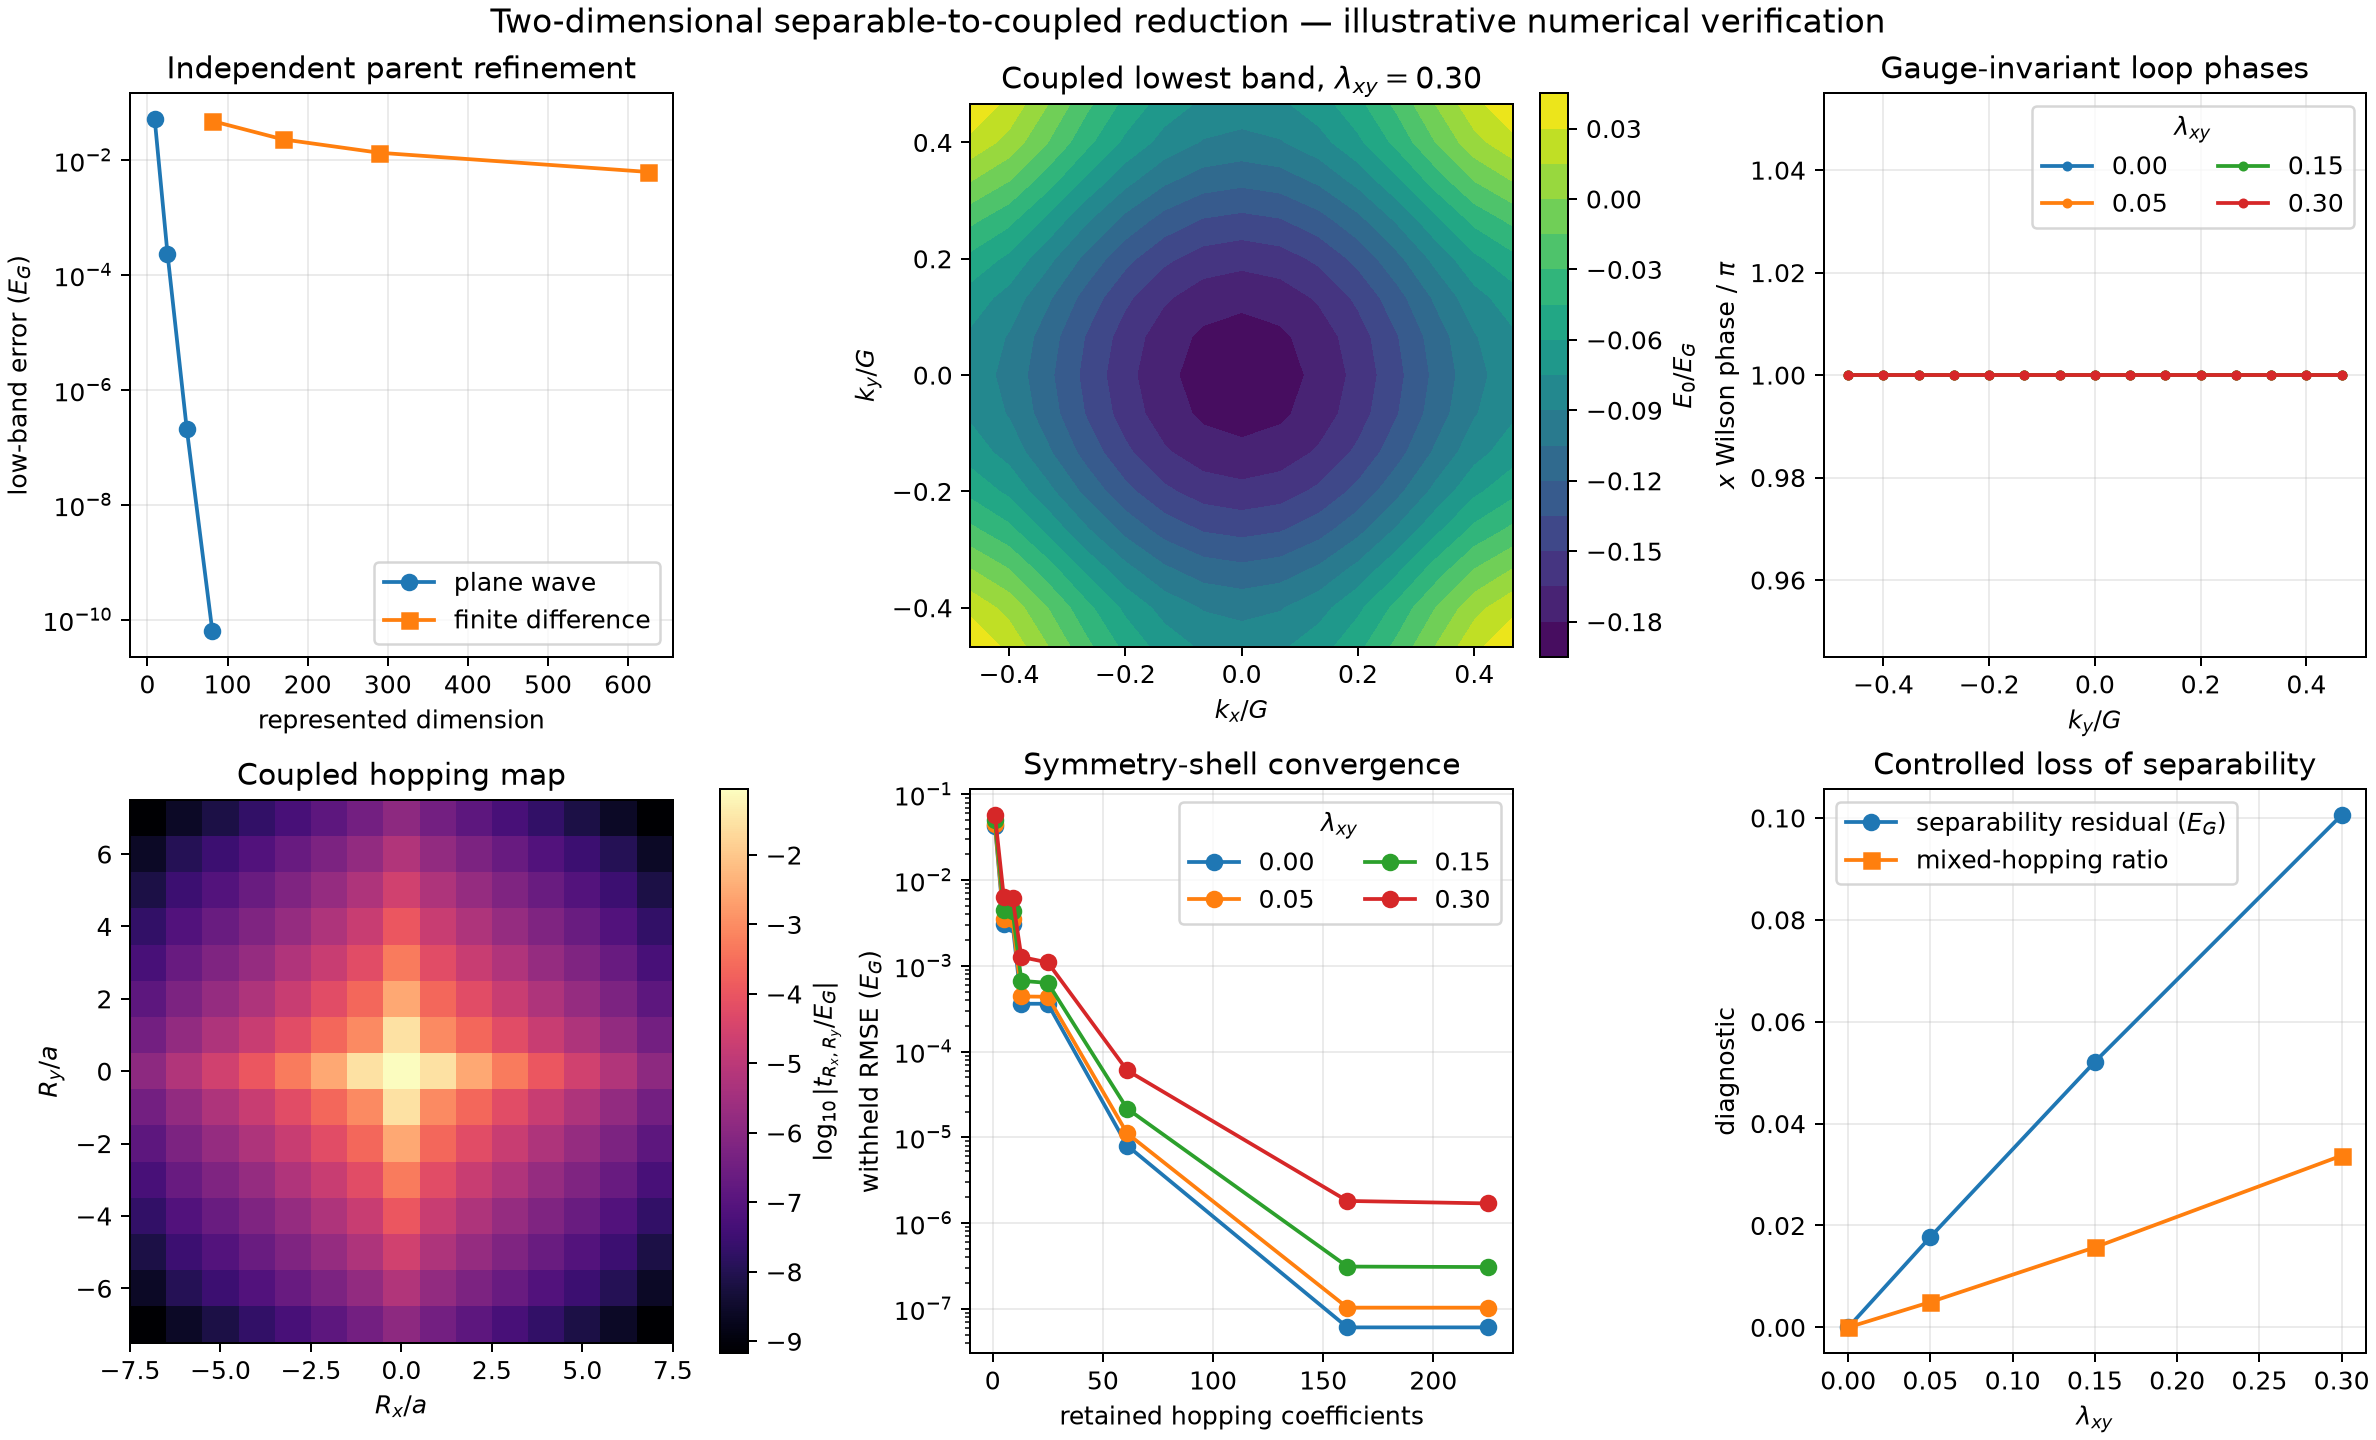
\includegraphics[
    width=\textwidth,
    height=0.82\textheight,
    keepaspectratio
  ]{../../../calculations/research-monograph/periodic-2d/summary.png}
  \caption{Calculated two-dimensional controlled exercise. The panels retain
  parent-representation refinement, the full coupled lowest-band surface,
  gauge-invariant Wilson phases, the mixed-direction hopping map, frozen
  symmetry-shell convergence, and the controlled loss of separability. The
  plotted results are illustrative numerical verification, not material
  validation.}
  \label{fig:periodic-2d-summary}
\end{figure}

The independently implemented verifier reconstructs the parent matrices,
separable spectra and projector, all retained mesh energies, reciprocal-boundary
sewing, Chern sum, hoppings, shell fits, withheld errors, and mass tensors
without importing the runner. It reports zero serialized-energy and hopping
reconstruction defect at the retained binary64 precision. The complete
reproduction package is retained under
\path{calculations/research-monograph/periodic-2d/}.

\subsection{Rank-three composite extension}

At $\lambda_{xy}=0.15$, the lowest three bands remain separated from the
exterior by at least $3.48\times10^{-2}E_G$. Projection of centered Gaussian
$s$, $p_x$, and $p_y$ trials has minimum singular value 0.886, while the minimum
sewn-neighbor singular value is 0.785. These controls establish a full-rank
direct projected frame on the declared mesh; they do not establish a preferred
material-orbital choice.

A deterministic rapidly varying internal $O(3)$ rotation supplies a rough gauge
without changing the retained projector. Smooth and rough frames agree in mesh
spectra within $1.22\times10^{-15}E_G$, in branch-aware Wilson eigenphase sets
within $2.22\times10^{-15}$, and in zero total Chern number. They do not agree
in localization: the rough gauge raises the total finite-supercell spread from
$24.90a^2$ to $67.70a^2$. At squared-radius shell 18, the omitted hopping-block
norm rises from $1.38\times10^{-2}E_G$ to $5.25\times10^{-1}E_G$. Thus subspace
and topology diagnostics are invariant under the attack while represented
hopping locality is not.

Independent reconstruction of the external comparison exposed a provisional
direct-gauge error: multiplying the square trial-overlap matrix by its full
inverse had returned the raw eigengauge. The corrected frame uses the polar
factor $A(A^\dagger A)^{-1/2}$. The runner evaluates it by SVD, while the
independent verifier uses a Hermitian eigendecomposition. The correction changes
the gauge-coordinate diagnostics above but not the retained parent, projector,
gap, or gauge-invariant topology conclusions.

\begin{figure}[p]
  \centering
  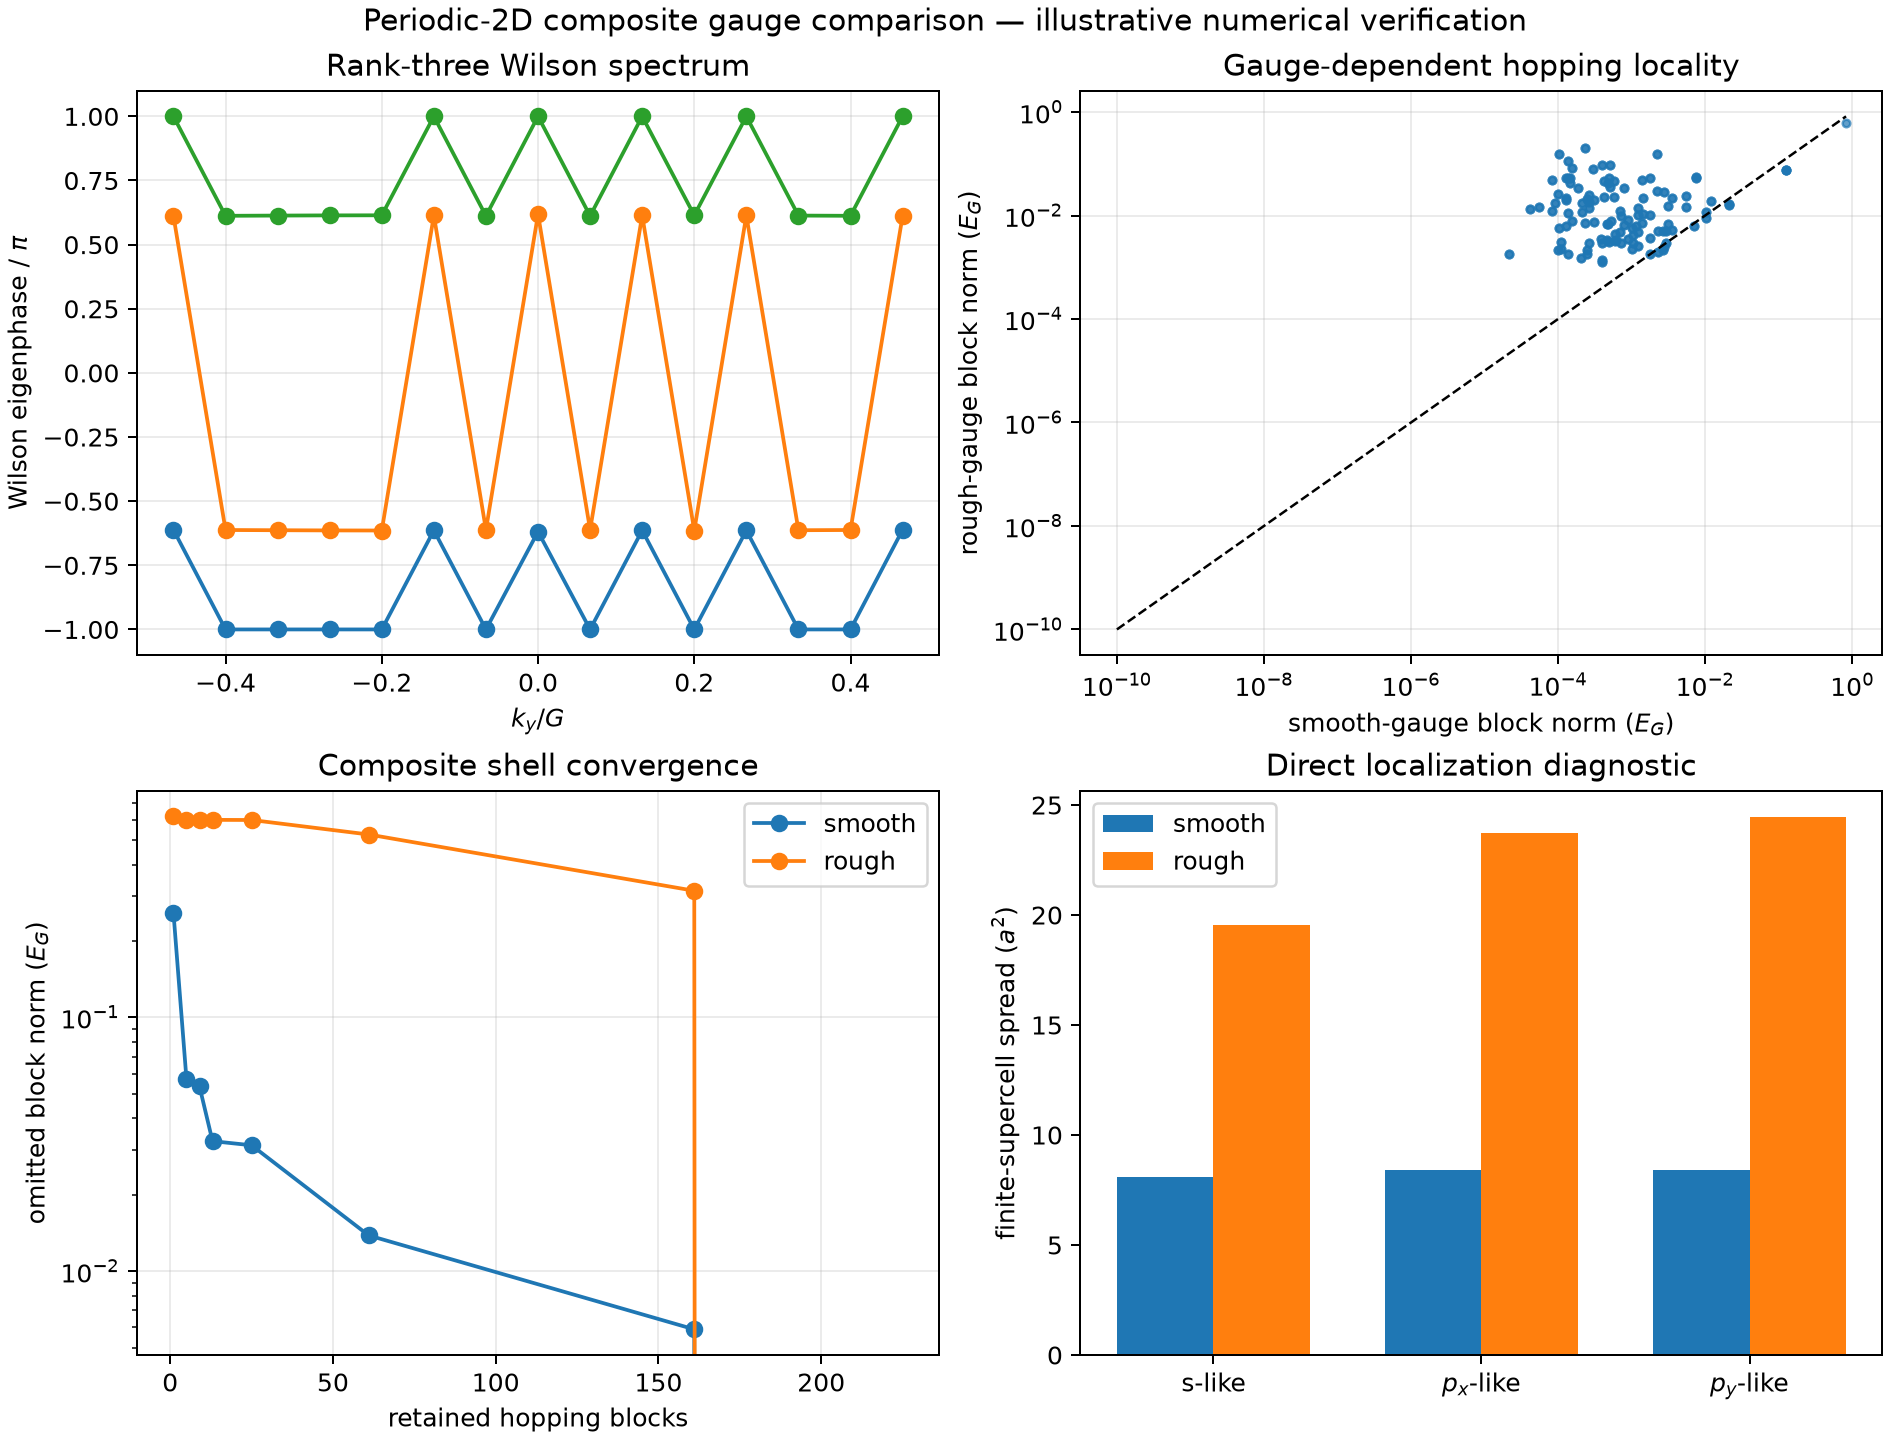
\includegraphics[
    width=\textwidth,
    height=0.82\textheight,
    keepaspectratio
  ]{../../../calculations/research-monograph/periodic-2d/composite-summary.png}
  \caption{Direct rank-three composite comparison. The Wilson spectrum and
  represented eigenvalues survive the internal gauge attack, whereas
  finite-supercell spreads and matrix-valued hopping locality worsen. The
  finite spreads are numerical diagnostics, not an infinite-mesh localization
  theorem.}
  \label{fig:periodic-2d-composite}
\end{figure}

The independent verifier reconstructs the trial projection, exterior gap,
non-Abelian links, determinant Chern sum, Wilson spectra, hopping blocks, shell
errors, density identities, and spreads without importing the runner. No
independent Wannier90 result is inferred from this direct comparison.

\subsection{Retained failure and corrected Wannier90 comparison}

The single authorized Wannier90 3.1.0 attempt stopped during preprocessing with
\texttt{kmesh\_get: something wrong, found too many nearest neighbours}. It
exited with code 1 after 0.31~s and used 22,118,400 bytes maximum resident
memory. No \texttt{.nnkp} was emitted; therefore the \texttt{.mmn} interface
and localization stages were not started. The failure was retained without an
automatic retry.

The $15\times15\times1$ reciprocal mesh had been embedded in an auxiliary unit
cubic cell. Its inactive reciprocal increment is 15 times the active increments,
so Wannier90's three-dimensional completeness search encounters too many shorter
in-plane shells before reaching the inactive direction and exceeds its compiled
12-neighbor limit. This is an interface-embedding failure, not a spread-
minimization result or evidence against localization.

A separately authorized correction changed only the inactive direct-lattice
length from 1 to 15, balancing the reciprocal increments while preserving the
active parent, mesh, rank, projections, and localization controls. Preprocessing
then found six axial neighbors in 0.28~s, and localization converged in 94
iterations and 0.47~s with maximum resident memory 27.3~MB.

\begin{figure}[p]
  \centering
  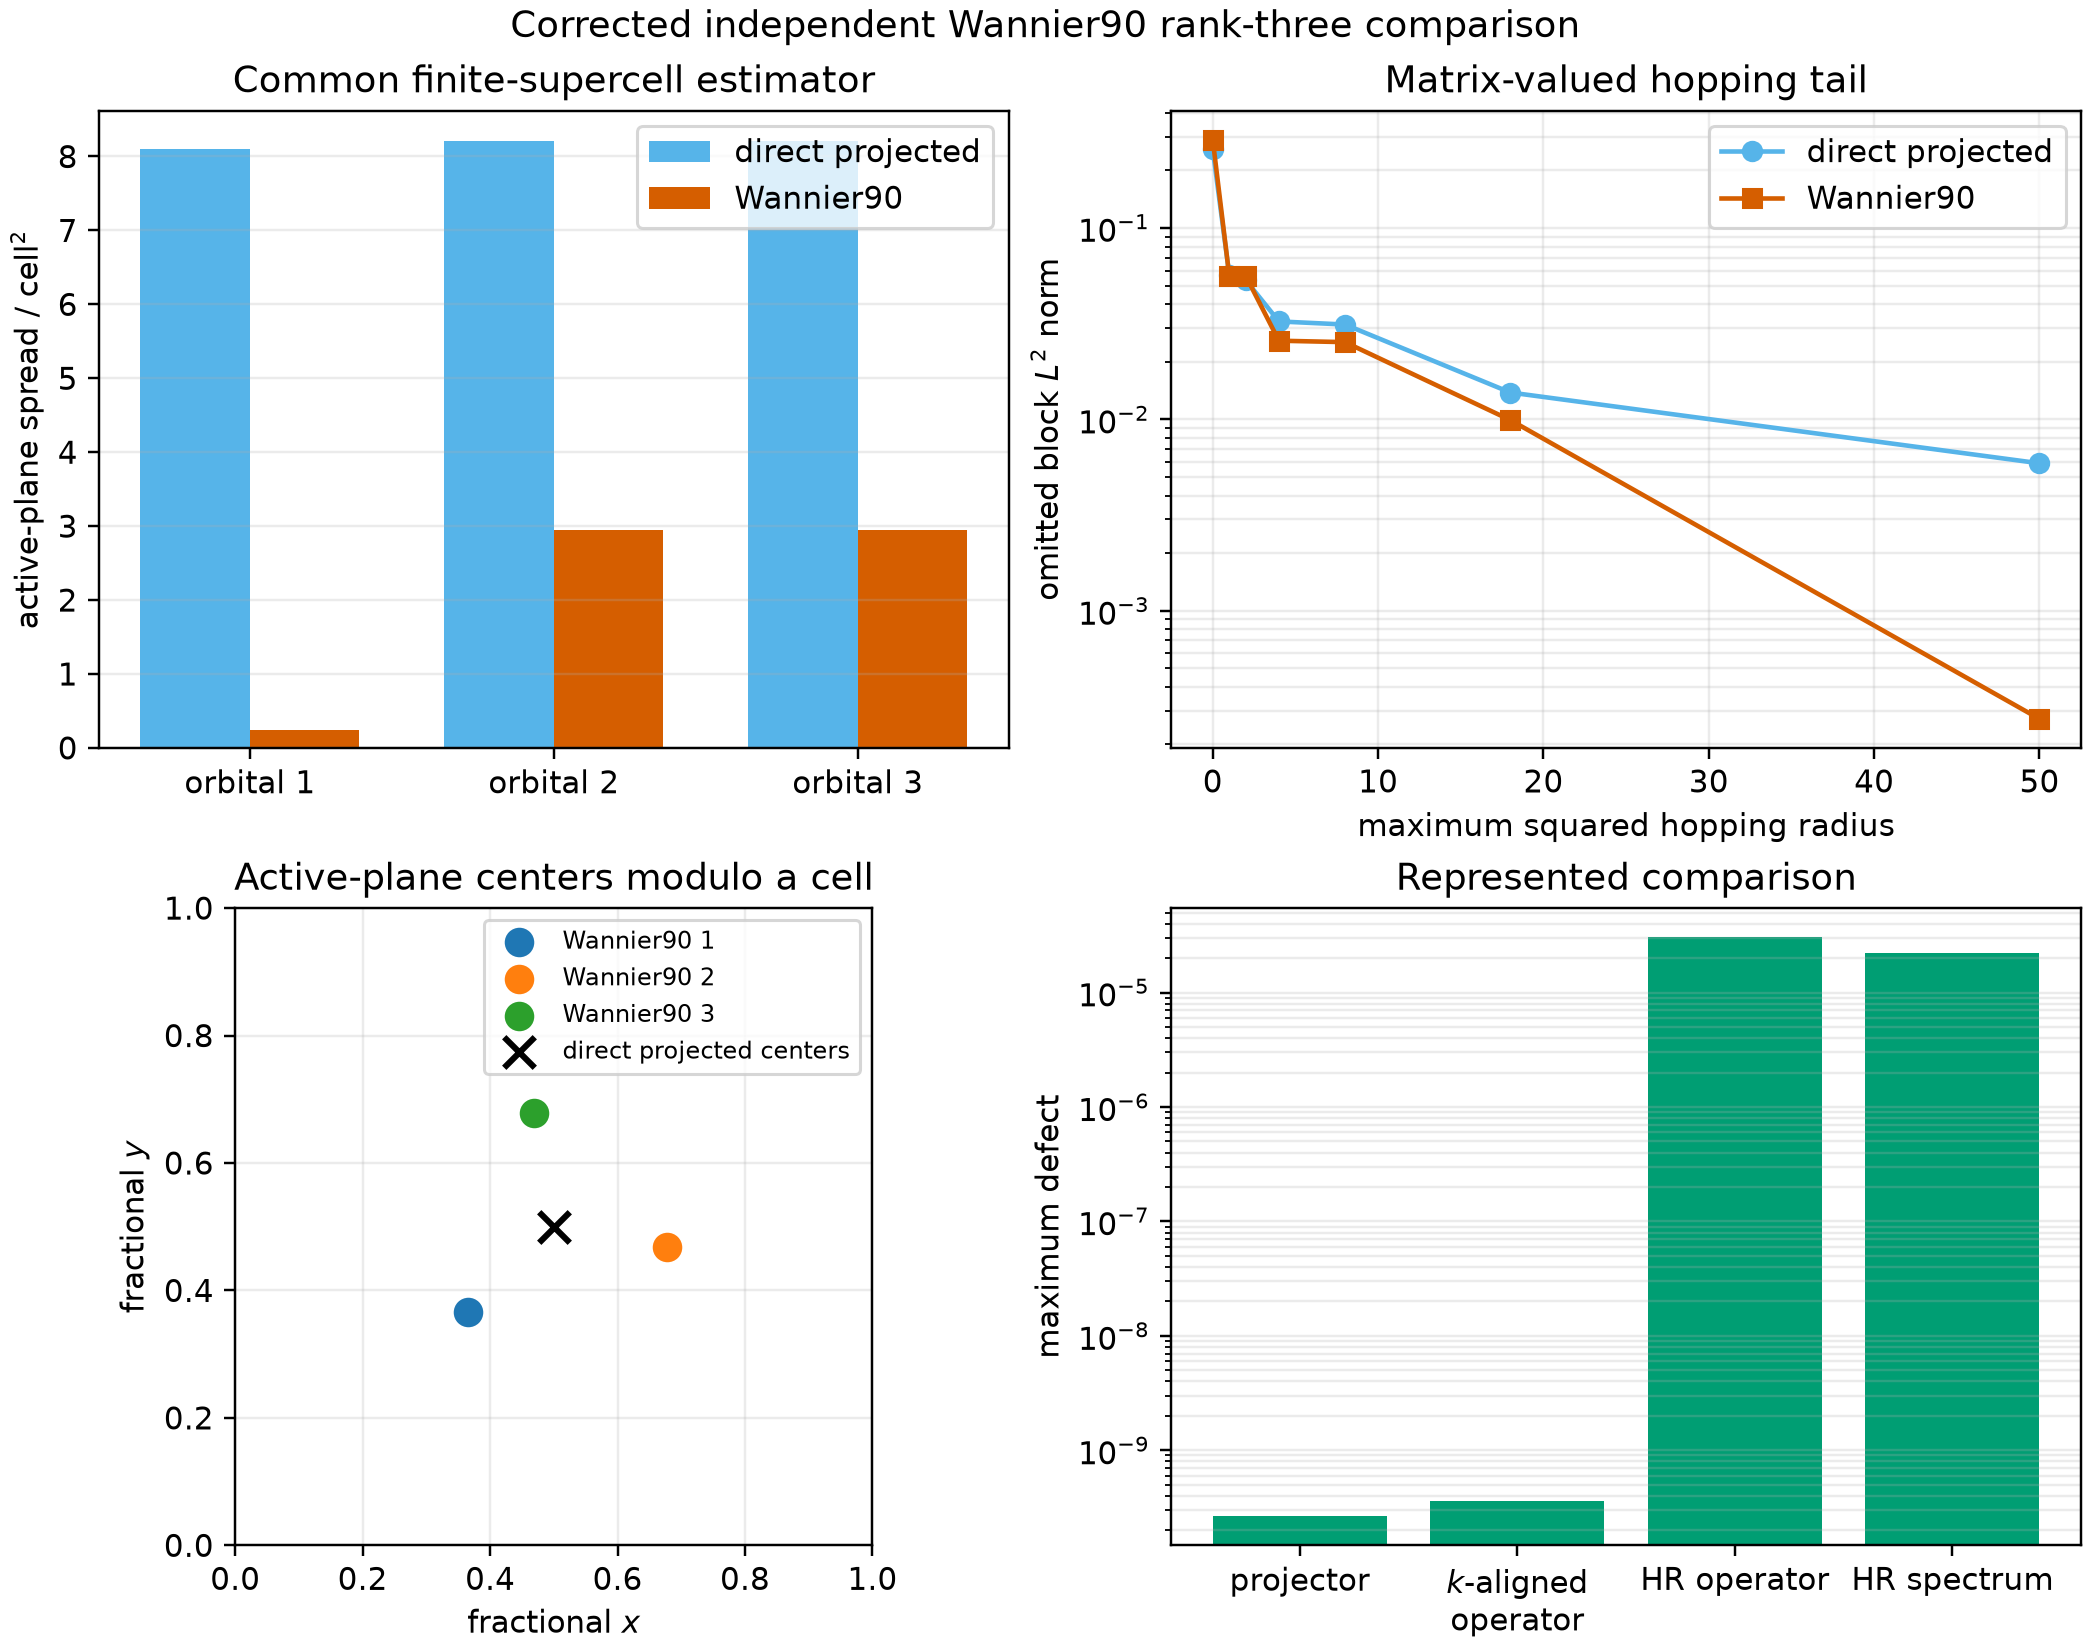
\includegraphics[
    width=\textwidth,
    height=0.82\textheight,
    keepaspectratio
  ]{../../../calculations/research-monograph/periodic-2d/wannier90-balanced-summary.png}
  \caption{Corrected independent Wannier90 rank-three comparison. On one common
  finite-supercell estimator, external spread minimization reduces active-plane
  spread and the long-range hopping tail. Projector and aligned-operator defects reflect printed
  $U$-matrix precision; the larger \texttt{\_hr.dat} defects reflect its
  six-decimal serialization.}
  \label{fig:periodic-2d-wannier90-balanced}
\end{figure}

The native Berry-link spreads are $0.2072a^2$, $0.2509a^2$, and
$0.2513a^2$, totaling $0.7094a^2$. They are not directly substituted for the
direct route's finite-supercell estimator. Reconstructing the Wannier90 frame
on the same $128^2$ grid gives spreads $0.2358a^2$, $2.9532a^2$, and
$2.9469a^2$, totaling $6.1359a^2$, versus $24.5163a^2$ for the corrected direct
projected frame reconstructed from that same external mesh. The separate
centered-mesh direct route gives $24.8951a^2$. At squared-radius shell 50, the
omitted hopping norm decreases from $5.90\times10^{-3}E_G$ to
$2.72\times10^{-4}E_G$. The native/common-estimator discrepancy is retained as
an estimator/discretization difference, not a localization gain. The frames span the same
retained subspace within $2.65\times10^{-10}$; exact $k$-dependent alignment
reduces their represented-operator defect to $3.57\times10^{-10}E_G$.

A bounded search over integer translations in $[-1,1]^2$ for each orbital and
one constant unitary leaves a per-orbital frame RMS defect of 1.188. Thus the
optimized gauge is not merely a translated or constantly rotated copy of the
direct projected frame. Native hopping blocks reconstruct the mesh within
$3.06\times10^{-5}E_G$ in Frobenius norm and $2.23\times10^{-5}E_G$
spectrally, retained separately as decimal serialization error. An independent
verifier reconstructs the parent, polar frame, bounded alignment, native
hoppings, common-grid densities, spreads, and shell tails without importing the
extractor. A compact extracted numerical fixture retained with the result makes
these reconstructions repository-portable; native-file identity, format, and
execution-log checks remain a stronger mode requiring the external run.

\subsection{Three distinct topological controls}

The topological extension keeps three finite-dimensional Bloch models separate:
the two-state Qi--Wu--Zhang model~\cite{qiWuZhang2006}, the three-state
flux-$1/3$ Hofstadter magnetic cell~\cite{hofstadter1976}, and the two-state
periodic-gauge Haldane model~\cite{haldane1988}. The magnetic-band Chern
interpretation follows the Thouless--Kohmoto--Nightingale--den Nijs
construction~\cite{thoulessKohmotoNightingaleDenNijs1982}. Each model has a
declared topological parameter and a declared trivial control. None is a
representation or approximation of the scalar continuum cosine operator, and
their numerical errors and energy units are not combined.

For the implemented Qi--Wu--Zhang convention, gap closings occur at
$m=-2,0,2$; the selected $m=-1$ case lies in the lower-band $C=-1$ interval,
whereas $m=3$ is analytically trivial. For Haldane, the selected masses are
separated by the analytic boundary
$|M|=3\sqrt{3}|t_2\sin\phi|\simeq0.7794$: $M=0$ is topological and $M=1$ is
trivial. At Hofstadter flux $1/3$, the Diophantine assignment gives
$(-1,+2,-1)$ in the orientation used here. The finite $\Delta=4$
atomic-superlattice case remains a declared numerical negative control; no
analytic transition threshold is claimed for that value.

On each mesh $N=21,31,51,81$, normalized neighbor links define plaquette Chern
sums and horizontal Wilson phases. At $N=81$, the topological retained gaps are
2.000, 1.274, and 1.559 in the respective model units. Every topological lower
band has Chern integer $-1$ and Wilson winding $+1$ on every mesh. The full-band
Chern tuples are $(-1,+1)$ for Qi--Wu--Zhang and Haldane and
$(-1,+2,-1)$ for Hofstadter. Every declared trivial control has zero retained
Chern sum and zero winding.

\begin{figure}[p]
  \centering
  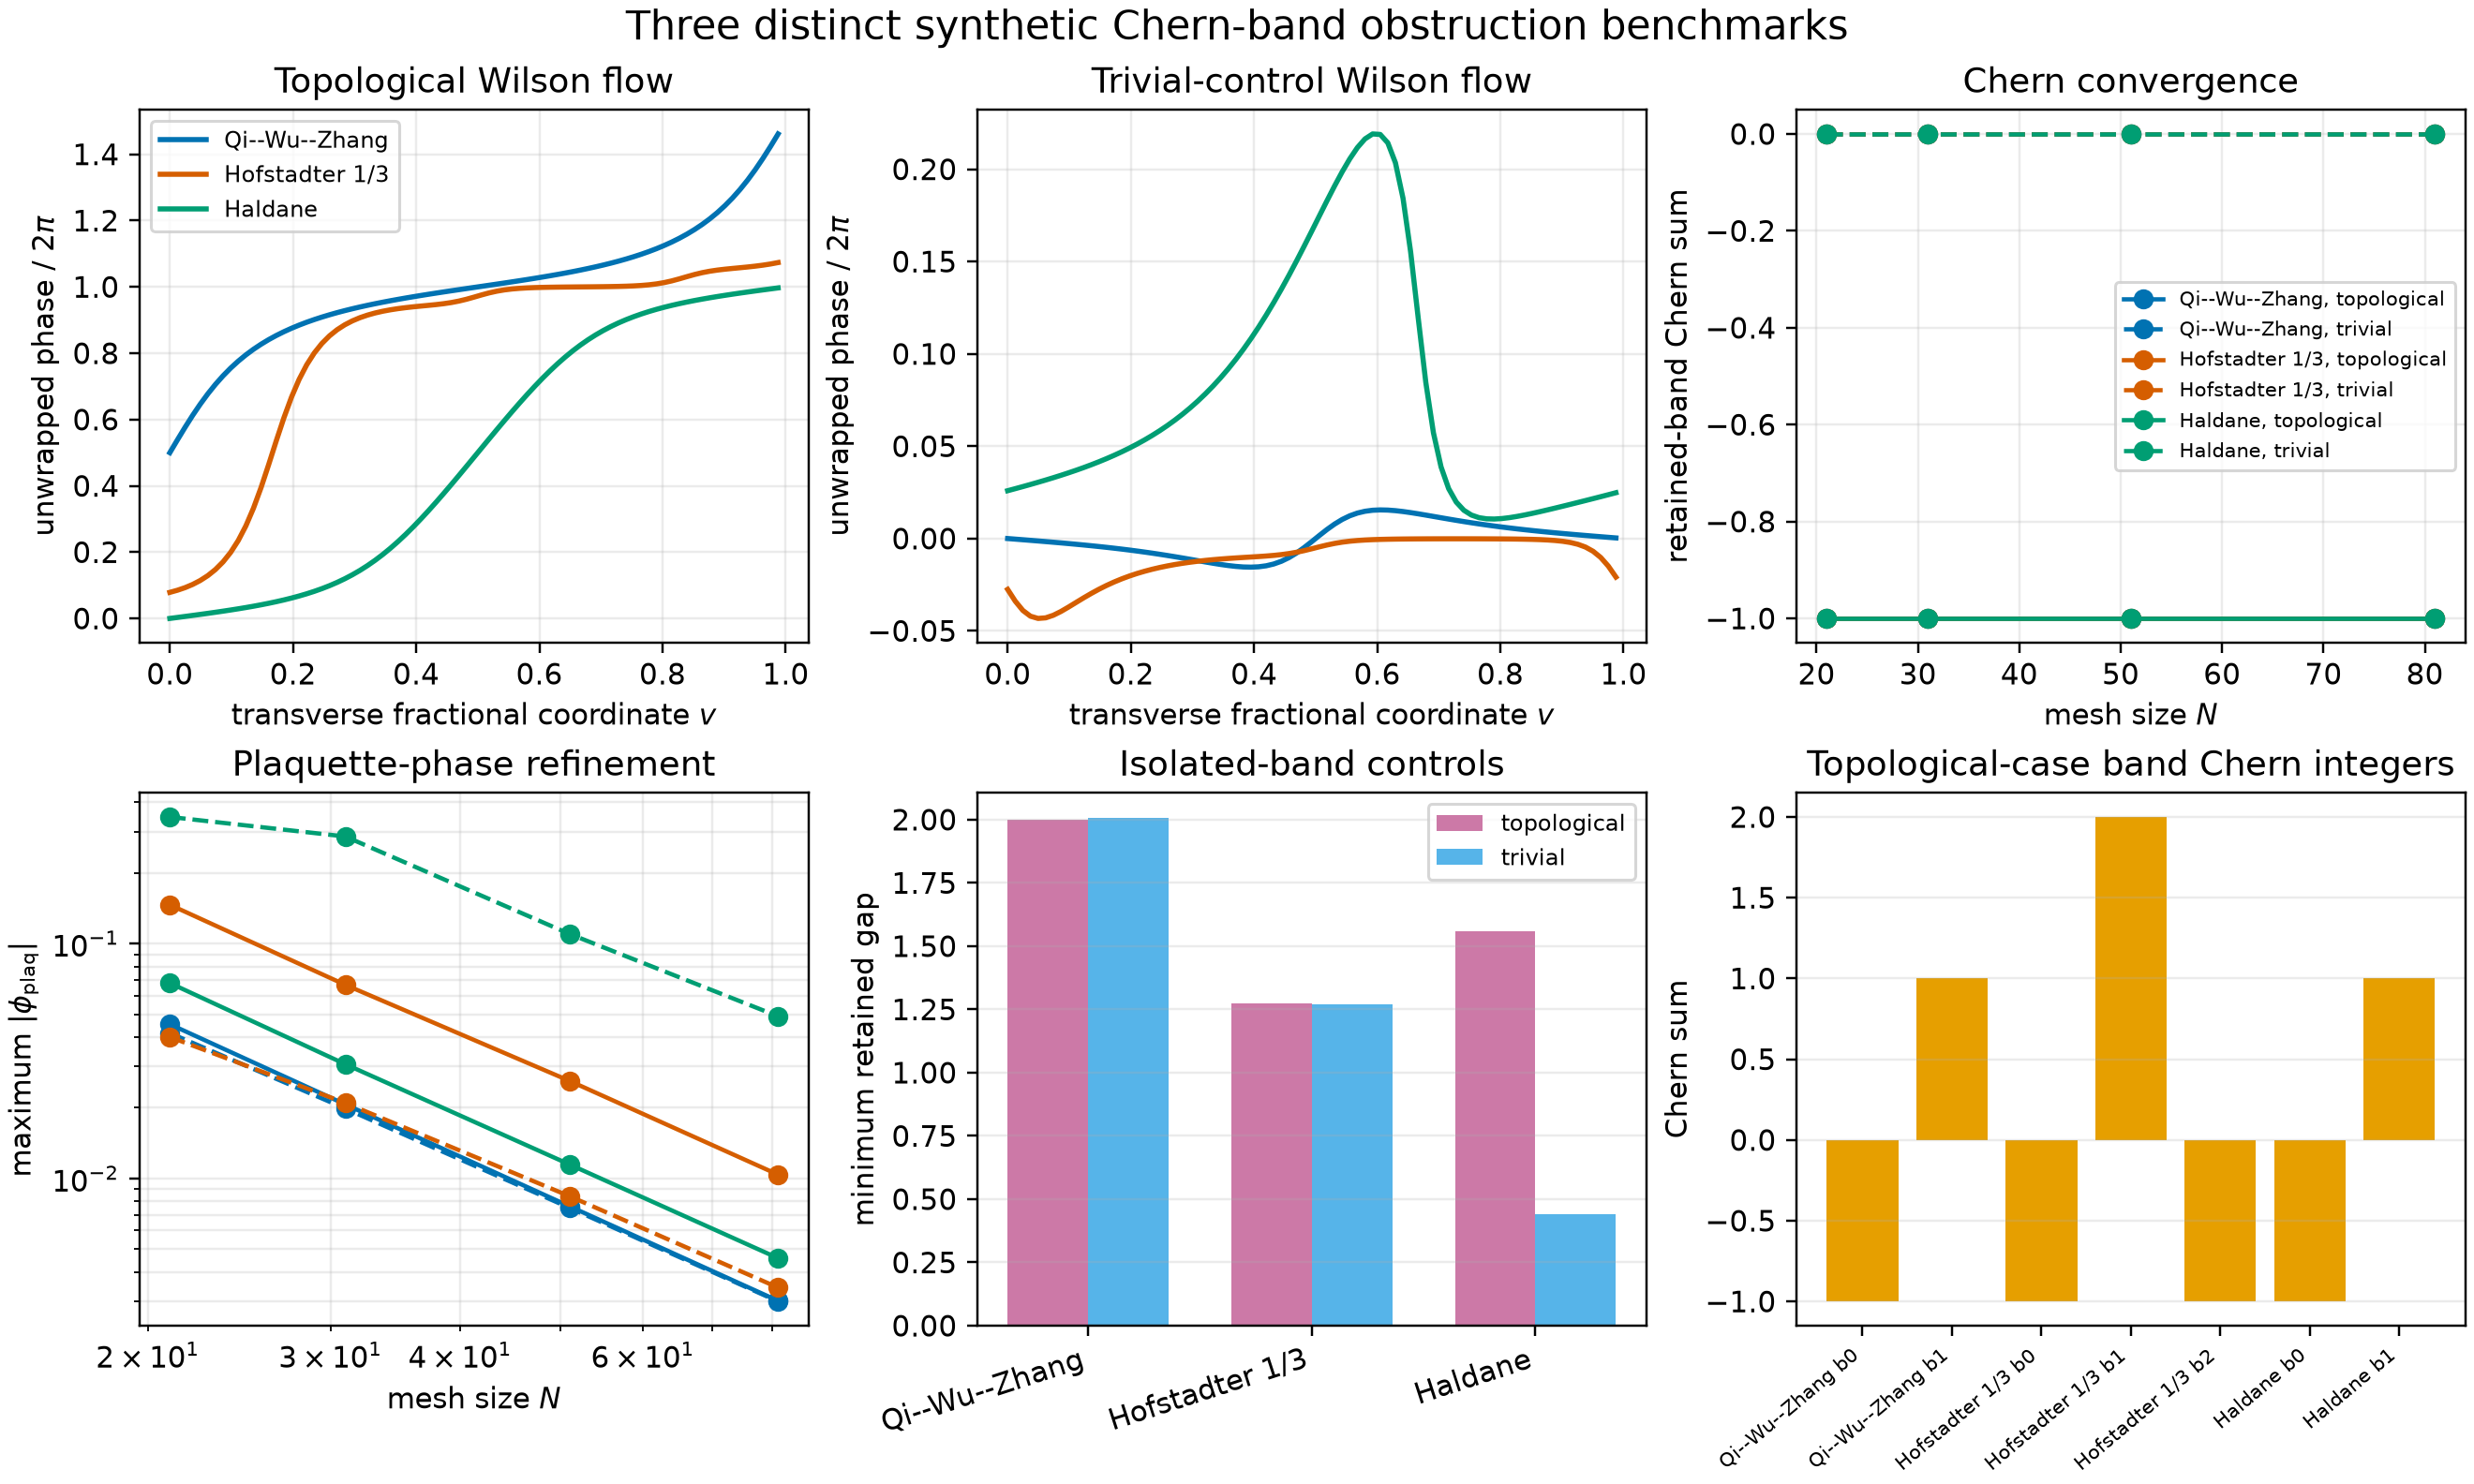
\includegraphics[
    width=\textwidth,
    height=0.82\textheight,
    keepaspectratio
  ]{../../../calculations/research-monograph/periodic-2d/topological-summary.png}
  \caption{Three separate synthetic Chern-band controls. Nonzero Chern sums
  and Wilson winding persist under mesh refinement in each topological case;
  the declared trivial controls remain at zero. Model-specific gaps and errors
  are not combined.}
  \label{fig:periodic-2d-topological}
\end{figure}

A deterministic periodic phase attack changes a Chern sum by at most
$2.3\times10^{-16}$ and a Wilson phase by at most
$1.5\times10^{-15}$. Reciprocal-seam projector defects remain below
$1.9\times10^{-15}$. The independent verifier reconstructs every Bloch matrix
and uses projector Bargmann products rather than the runner's normalized-link
route.

The nonzero Chern integer and Wilson winding evaluate the numerical premises of
the standard rank-one Wannier obstruction \cite{brouder2007}. They do not prove
the general theorem, establish topology for the scalar parent, or validate a
material. The complete separate contracts and limitations are retained in
\path{calculations/research-monograph/periodic-2d/topological-report.md}.

\subsection{Bounded non-DFT Wannier90 sensitivity study}

Six additional one-attempt cases vary reciprocal mesh, plane-wave cutoff, and
inactive embedding around $(P,N,c)=(3,15,15)$. All complete within their
retained resource limits, but the results are nonmonotone. The common
finite-supercell spread is $4.6847a^2$, $6.1359a^2$, and $8.4973a^2$ at
$N=11,15,19$, respectively. At $P=2$ and $P=4$ it is $9.3161a^2$ and
$10.3654a^2$, with radius-50 tails near $3.3\times10^{-2}E_G$ rather than the
reference $2.72\times10^{-4}E_G$.

\begin{figure}[p]
  \centering
  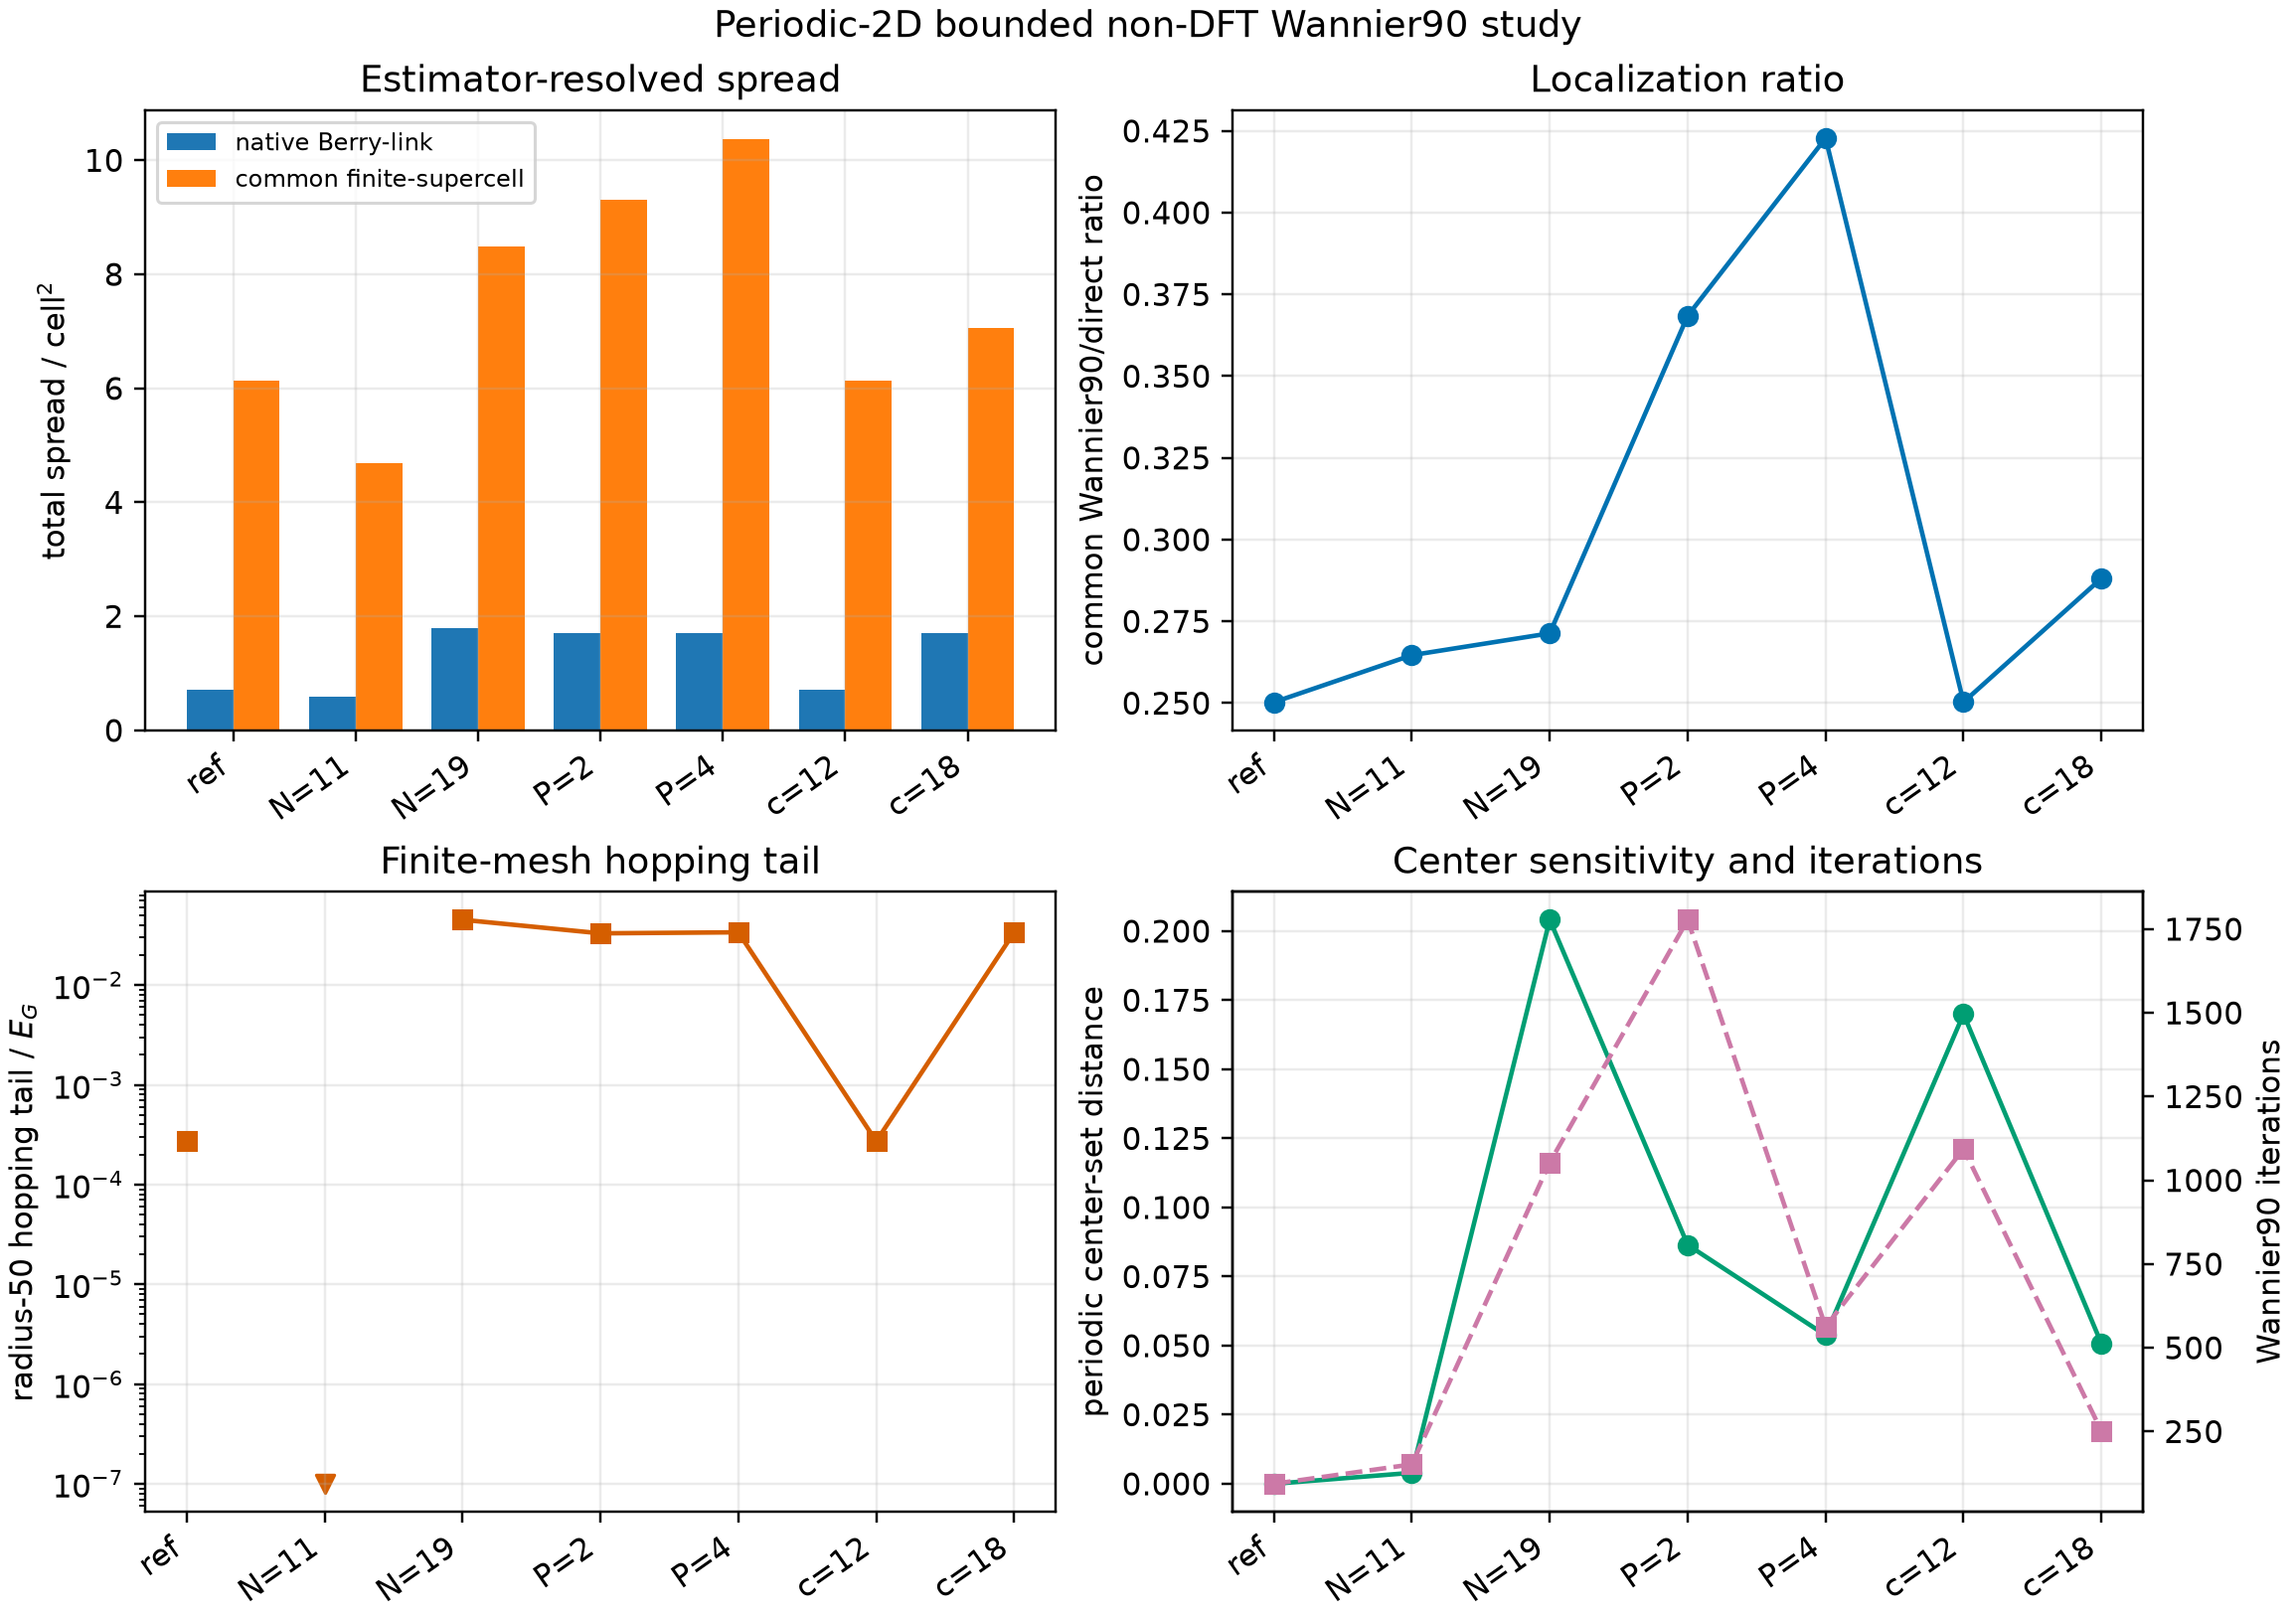
\includegraphics[
    width=\textwidth,
    height=0.82\textheight,
    keepaspectratio
  ]{../../../calculations/research-monograph/periodic-2d/wannier90-study-summary.png}
  \caption{Bounded non-DFT Wannier90 study. Native and common-estimator
  spreads, localization ratios, hopping tails, center-set sensitivity, and
  optimizer iterations are retained separately. The nonmonotone records do not
  establish a converged localization limit.}
  \label{fig:periodic-2d-wannier90-study}
\end{figure}

Changing only the inactive length to $c=12$ closely reproduces the reference
total spreads and tail, whereas $c=18$ converges to a different basin. Thus the
selected localized gauge is not demonstrated to be cutoff, mesh, or
embedding independent. No less-localized case is discarded and no retry or
alternative initialization is used to select a preferred outcome. A
checksummed local archive contains the native failure, reference, and study
files; it is prepared evidence, not a published deposit or release.

\subsection{Separate topological phase sweeps}

On a $51^2$ mesh, separate sweeps recover the Qi--Wu--Zhang changes at
$m=-2,0,2$ and bracket the Haldane changes around the analytic boundaries
$M=\pm0.7794$. The Hofstadter lower-band Chern integer changes from $-1$ to
zero between $\Delta=1.8$ and $2.0$ and remains zero through the sampled
continuation to $\Delta=12$. This supplies a numerical basis for the declared
$\Delta=4$ control without claiming an exact analytic transition value.

\begin{figure}[p]
  \centering
  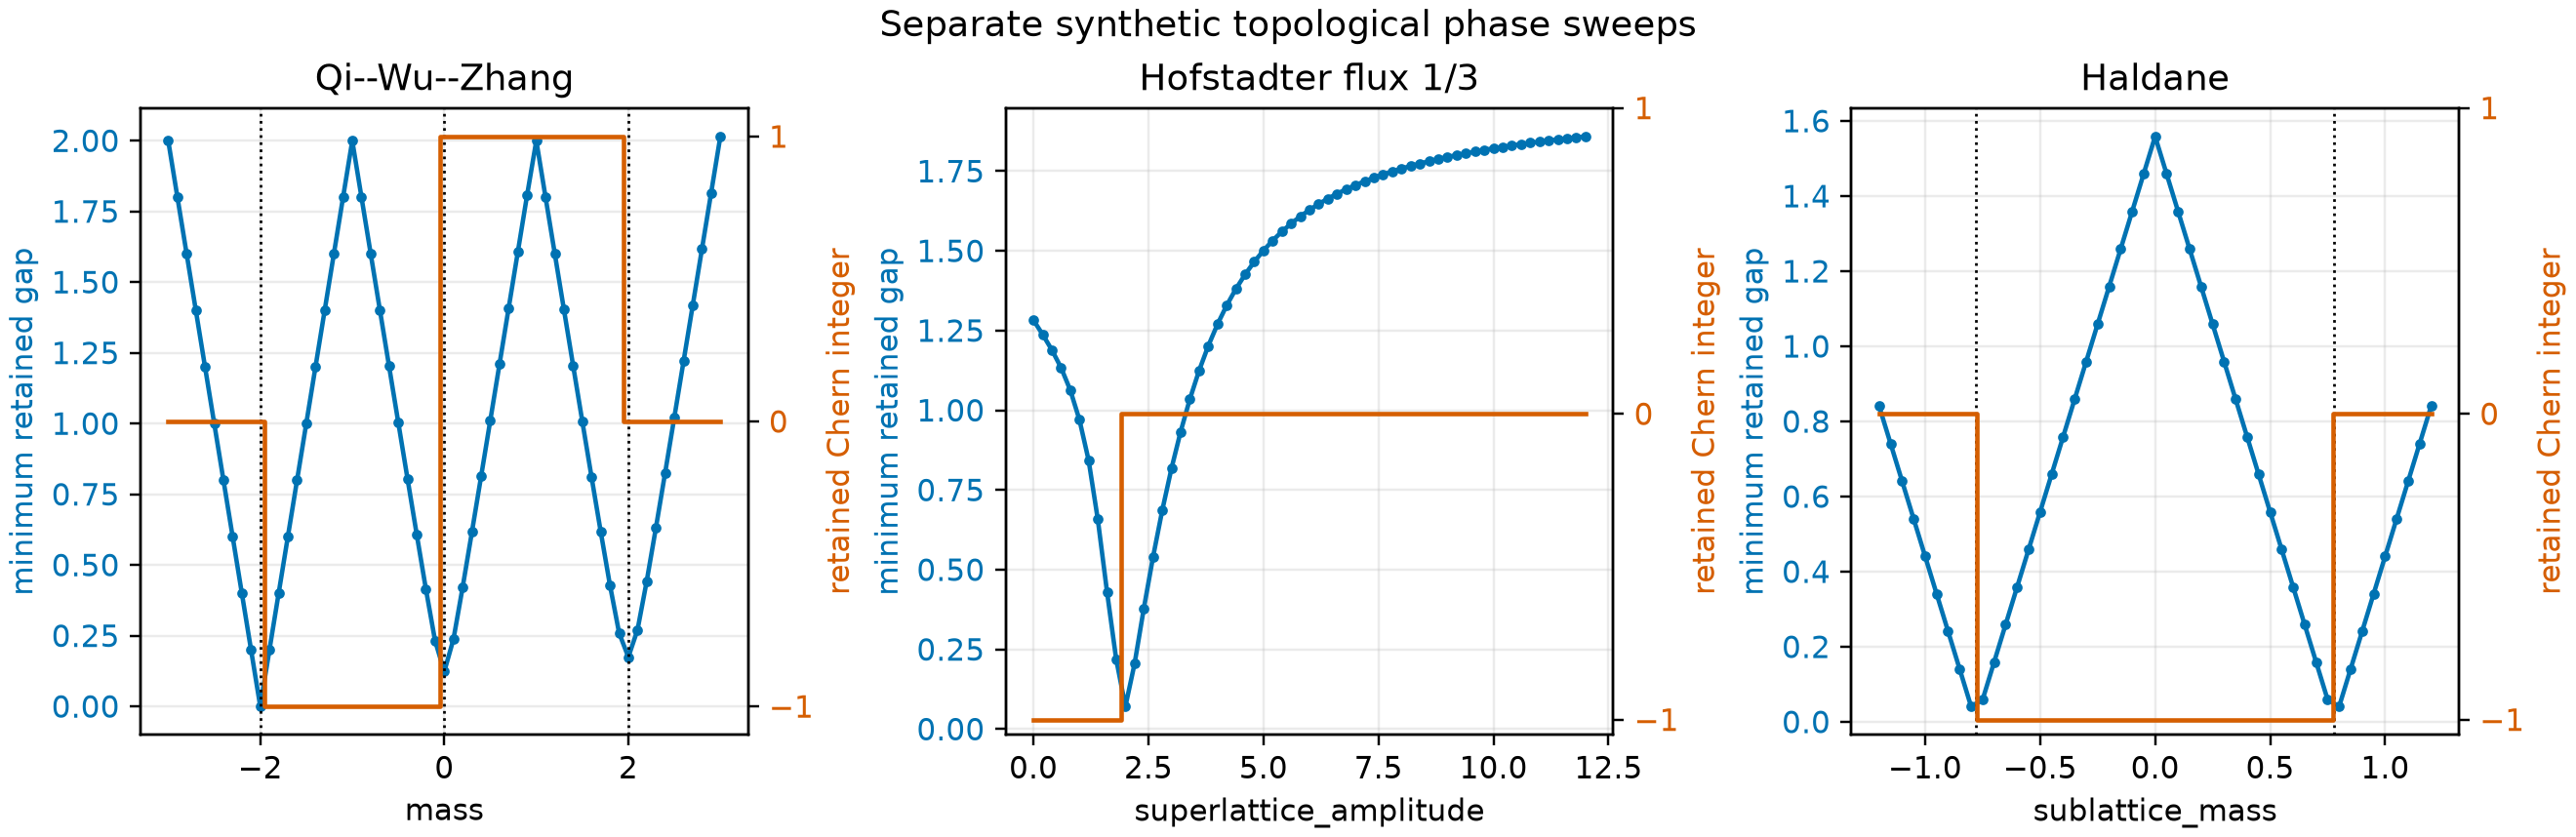
\includegraphics[
    width=\textwidth,
    height=0.82\textheight,
    keepaspectratio
  ]{../../../calculations/research-monograph/periodic-2d/topological-phase-sweep-summary.png}
  \caption{Separate synthetic topological parameter sweeps. Dotted boundaries
  are analytic only for Qi--Wu--Zhang and Haldane. Gaps and energy units remain
  model specific, and every sample is independently reconstructed through
  projector Bargmann loops.}
  \label{fig:periodic-2d-topological-phase-sweep}
\end{figure}

\section{Remaining plot opportunities}

Figures~\ref{fig:periodic-2d-summary}--\ref{fig:periodic-2d-topological-phase-sweep}
complete the compact journal-facing summary. The following more detailed plots
remain optional future analyses and are not calculated evidence in this task.

\begin{enumerate}
    \item \textbf{Placeholder---potential surfaces.} Plot the separable,
          anisotropic, and coupled potentials over several cells.
    \item \textbf{Placeholder---separable energy check.} Compare calculated
          two-dimensional energies with sums of one-dimensional energies over
          the reciprocal mesh.
    \item \textbf{Placeholder---product-state projector check.} Plot projector
          or principal-angle discrepancies between calculated and product
          subspaces, especially at degeneracies.
    \item \textbf{Placeholder---two-dimensional band surfaces.} Display
          selected $E_n(k_x,k_y)$ surfaces rather than only a high-symmetry
          path.
    \item \textbf{Placeholder---high-symmetry band path.} Plot
          $\Gamma$--$X$--$M$--$\Gamma$ overlays for the plane-wave, real-space,
          Wannier, and TB representations.
    \item \textbf{Placeholder---parent convergence maps.} Display spectral,
          projector, and low-sector Frobenius errors over
          $(P_x,P_y)$ and $(\Delta x/a,\Delta y/a)$.
    \item \textbf{Placeholder---matrix coupling structure.} Show reciprocal
          matrix heat maps distinguishing axis couplings from the diagonal
          couplings introduced by $V_{xy}$.
    \item \textbf{Placeholder---symmetry residuals.} Plot time-reversal,
          rotation, and reflection residuals over the full reciprocal mesh.
    \item \textbf{Placeholder---effective-mass ellipses.} Display the principal
          axes and eigenvalues of the effective-mass tensor for selected band
          extrema.
    \item \textbf{Placeholder---neighbor-overlap conditioning.} Plot overlap
          magnitudes or singular values in both reciprocal directions.
    \item \textbf{Placeholder---composite Wilson-loop phase surfaces.} Display
          non-Abelian eigenphase branches beyond the retained scalar summary.
    \item \textbf{Placeholder---curvature maps.} Display the spatially resolved
          discretized Berry curvature behind the completed integrated Chern
          convergence controls.
    \item \textbf{Placeholder---direct and Wannier90 density overlays.} Extend
          the completed center-and-spread comparison with aligned active-plane
          density contours.
    \item \textbf{Placeholder---Wannier interpolation.} Plot full-mesh and
          withheld-point interpolation errors.
    \item \textbf{Placeholder---hopping maps.} Display
          $\lVert\mathbf H_{\mathrm W}(\mathbf R)\rVert_{\mathrm F}$ on the
          two-dimensional lattice, grouped by symmetry shell.
    \item \textbf{Placeholder---shell convergence.} Plot operator, spectral,
          gap, bandwidth, and mass-tensor errors against retained shell.
    \item \textbf{Placeholder---Parseval check.} Compare omitted real-space
          block norms with reciprocal residual norms.
    \item \textbf{Placeholder---direct versus mediated routes.} Plot the route
          defect over reciprocal space and against shell complexity.
    \item \textbf{Placeholder---separability breaking.} Plot selected operator,
          localization, and hopping diagnostics against
          $|V_{xy}|/E_G$.
    \item \textbf{Placeholder---anisotropy scan.} Plot mass tensors, hopping
          decay, and localization diagnostics against $V_x/V_y$ with the
          remaining controls fixed.
\end{enumerate}
Each completed plot should identify the potential parameters, reciprocal and
real-space cutoffs, full reciprocal mesh, retained subspace, degeneracy
handling, gauge, topology diagnostic, localization route, hopping shell,
normalization, units, and evidentiary status. A placeholder is not a calculated
result.

\section{Interpretation boundary}

The separable model supplies an exact bridge from the one-dimensional warmup.
The coupled model introduces genuinely two-dimensional structure without
immediately invoking a material-specific parent. Direct gauge transport makes
loop closure and topology visible; the corrected Wannier90 run supplies an
independent localization route whose mesh, cutoff, and auxiliary-embedding
sensitivity is now explicit. The shell hierarchy introduces directional and
symmetry constraints absent in one dimension.

The completed scalar, composite, separately represented topological slices,
phase sweeps, and bounded Wannier90 sensitivity cases establish numerical
verification for their declared two-dimensional models
under recorded conditions. They do not validate a two-dimensional material,
determine an acceptable silicon Wannier subspace, show that the same hopping
hierarchy is adequate for the diamond lattice, or turn the synthetic Wannier90
comparison into production or material evidence. Their role is to expose two-dimensional failure modes
before the three-dimensional multiorbital bulk-silicon reduction is attempted.
